\documentclass{beamer}
\usetheme{}
\usecolortheme{dolphin}           
\useinnertheme{circles}
\setbeamertemplate{itemize items}[default]
\setbeamertemplate{enumerate items}[default]
\usepackage[T1]{fontenc}
\usepackage[utf8]{inputenc}
\usepackage{lmodern}
\usepackage{amsmath}
\usepackage{booktabs} 
\usepackage{graphicx}        
\usepackage{array}
\usepackage{color}
\makeatletter
\def\zapcolorreset{\let\reset@color\relax\ignorespaces}
\def\colorrows#1{\noalign{\aftergroup\zapcolorreset#1}\ignorespaces}
\makeatother
\graphicspath{{/home/swl/Dropbox/ucd/advanced_macro/figures/}} 
\setbeamertemplate{navigation symbols}{}
\setbeamertemplate{footline}[frame number]
%--------------------------------------
\title{Phillips curve}
\author{School of Economics, University College Dublin}
\date{Spring 2018}
\begin{document}

%--------------------------------------
\begin{frame}
 \titlepage
\end{frame}
%--------------------------------------

%--------------------------------------
\begin{frame}
  \begin{figure}
    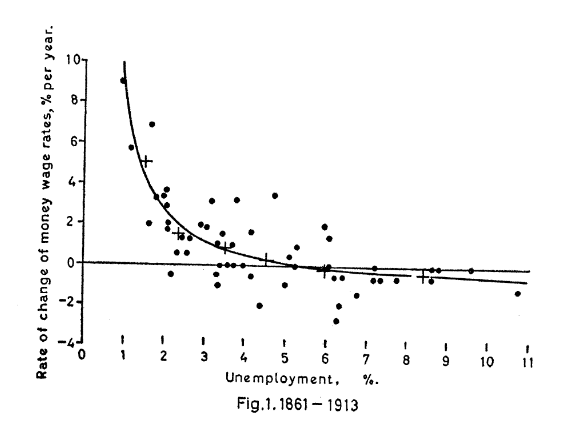
\includegraphics[scale=.8]{pc.eps}
  \end{figure}
\end{frame}
%--------------------------------------

%--------------------------------------
\begin{frame}
  \begin{figure}
    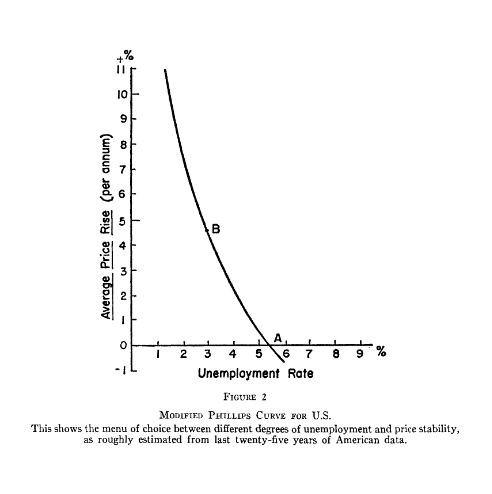
\includegraphics[scale=.8]{pc2.eps}
  \end{figure}
\end{frame}
%--------------------------------------

%--------------------------------------
\begin{frame}
  \begin{figure}
    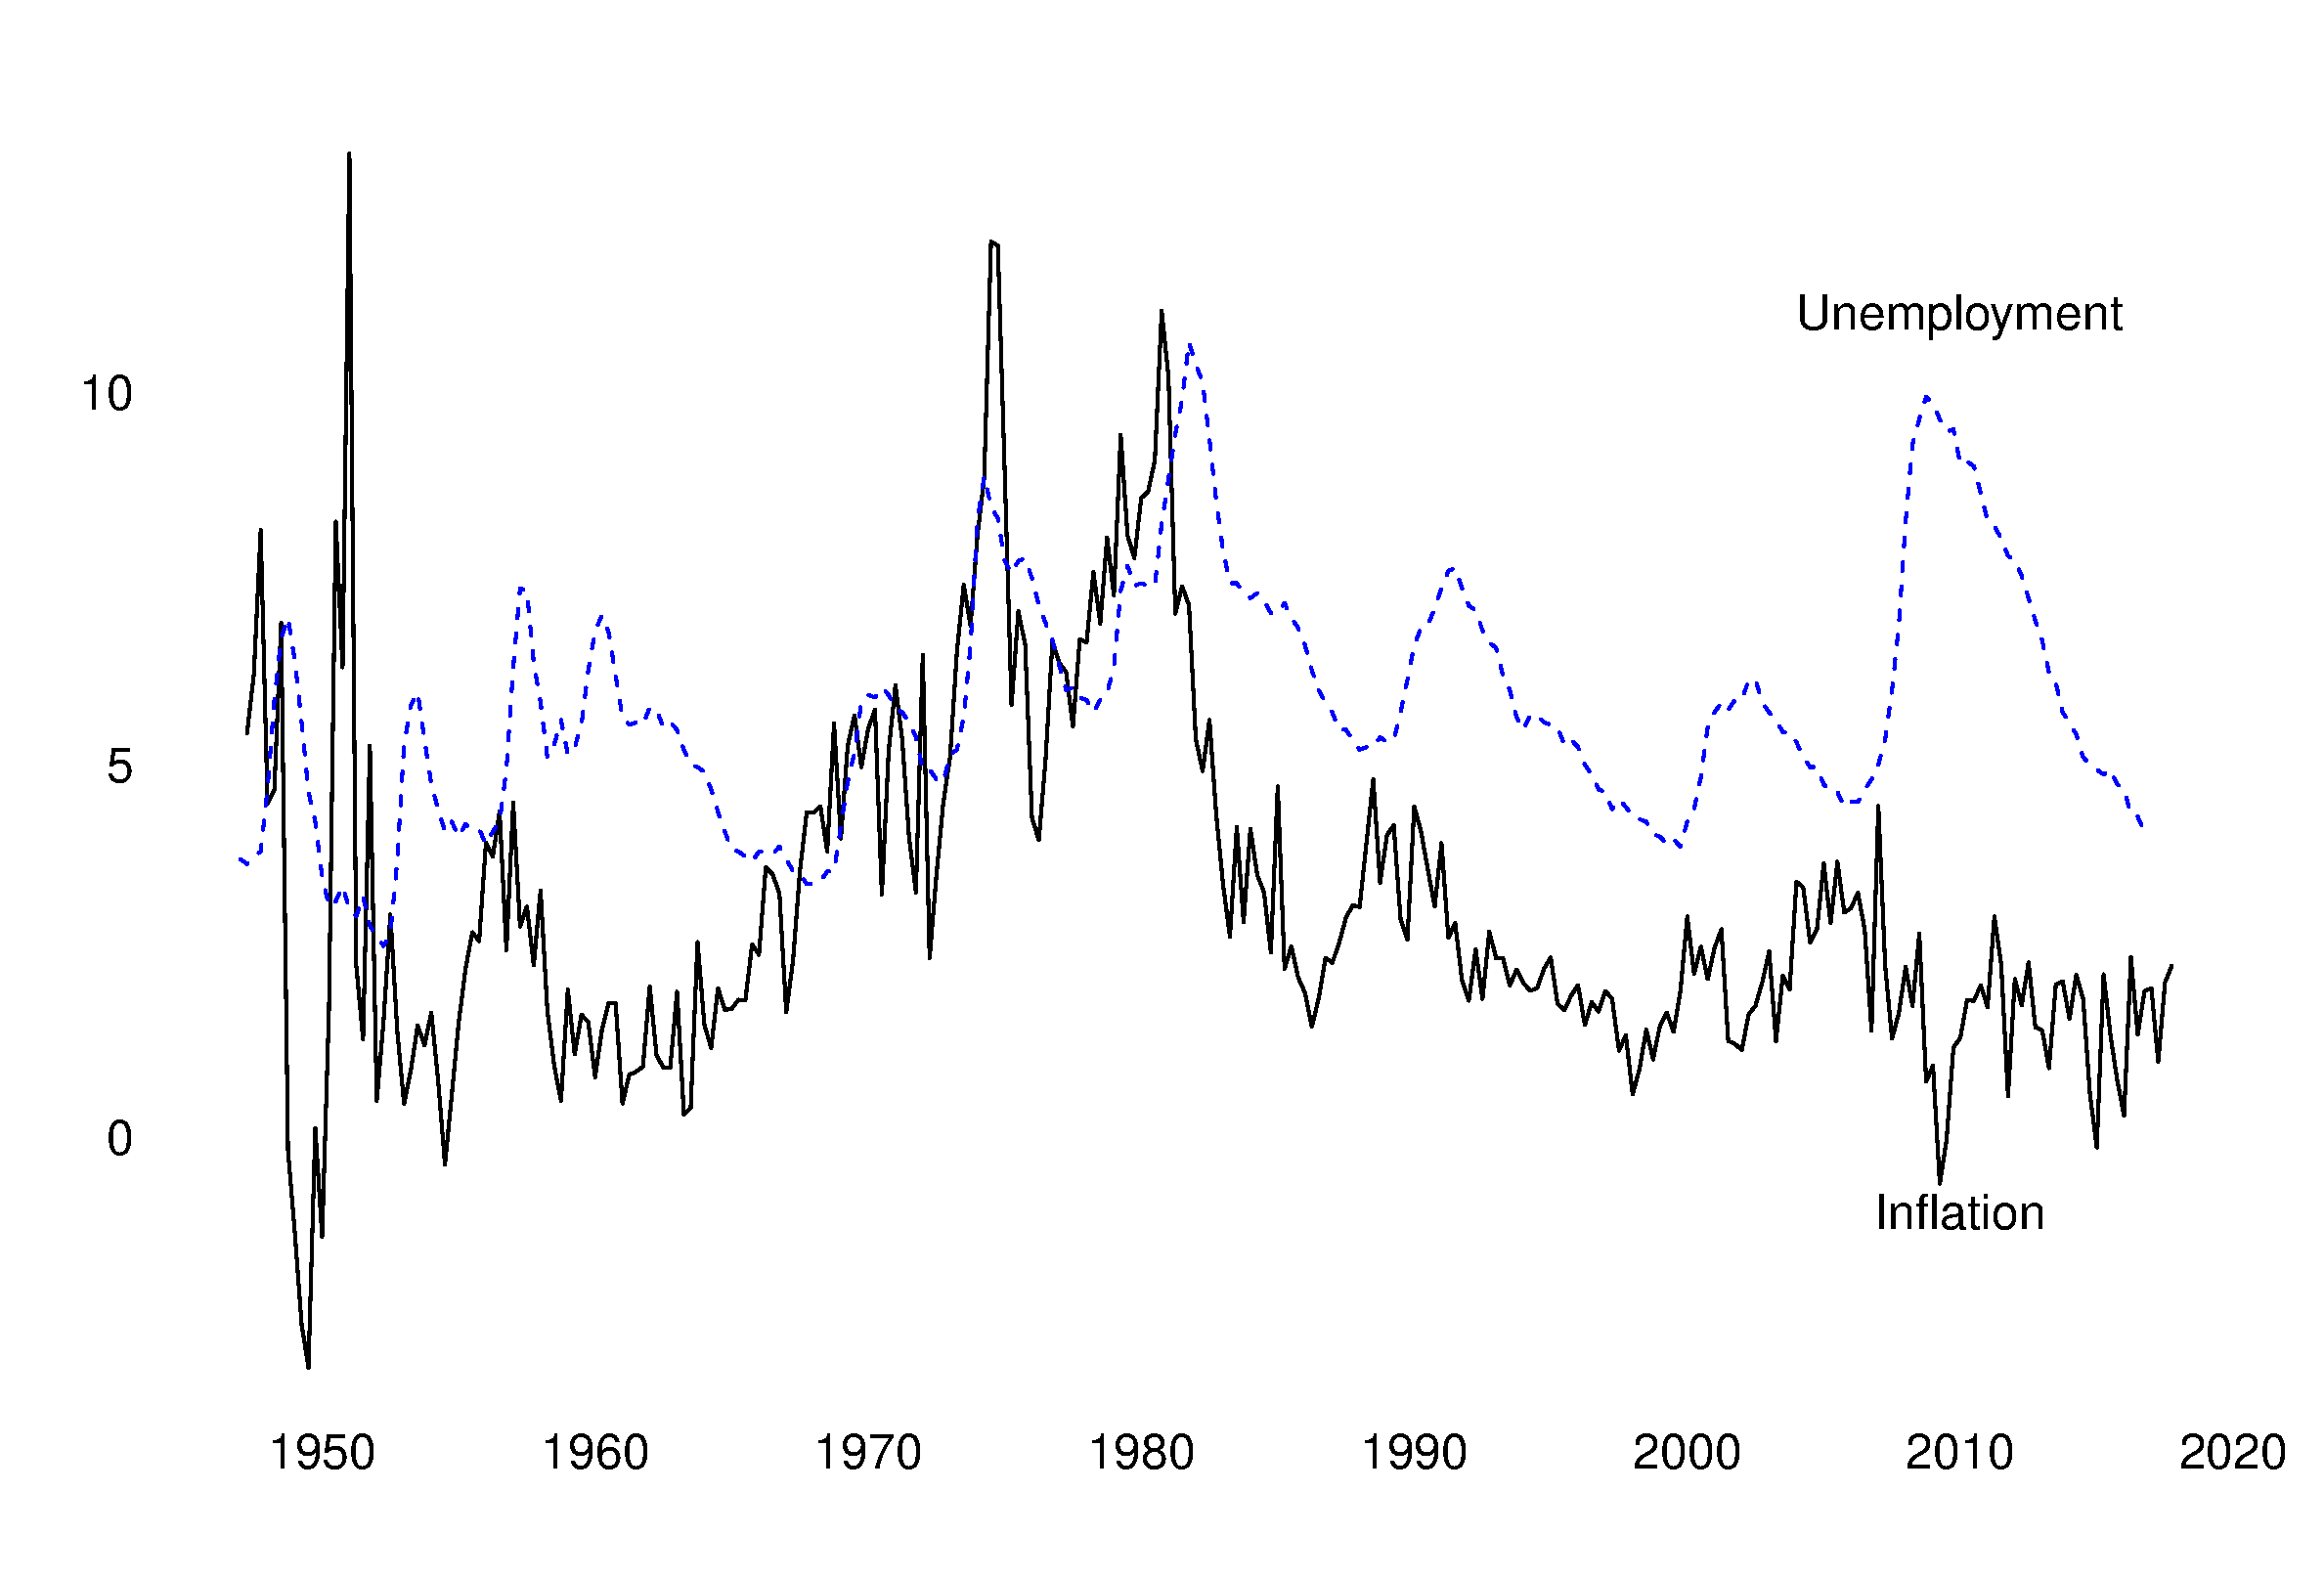
\includegraphics[scale=.25]{pc3.eps}
  \end{figure}
\end{frame}
%--------------------------------------

%--------------------------------------
\begin{frame}
  \begin{figure}
    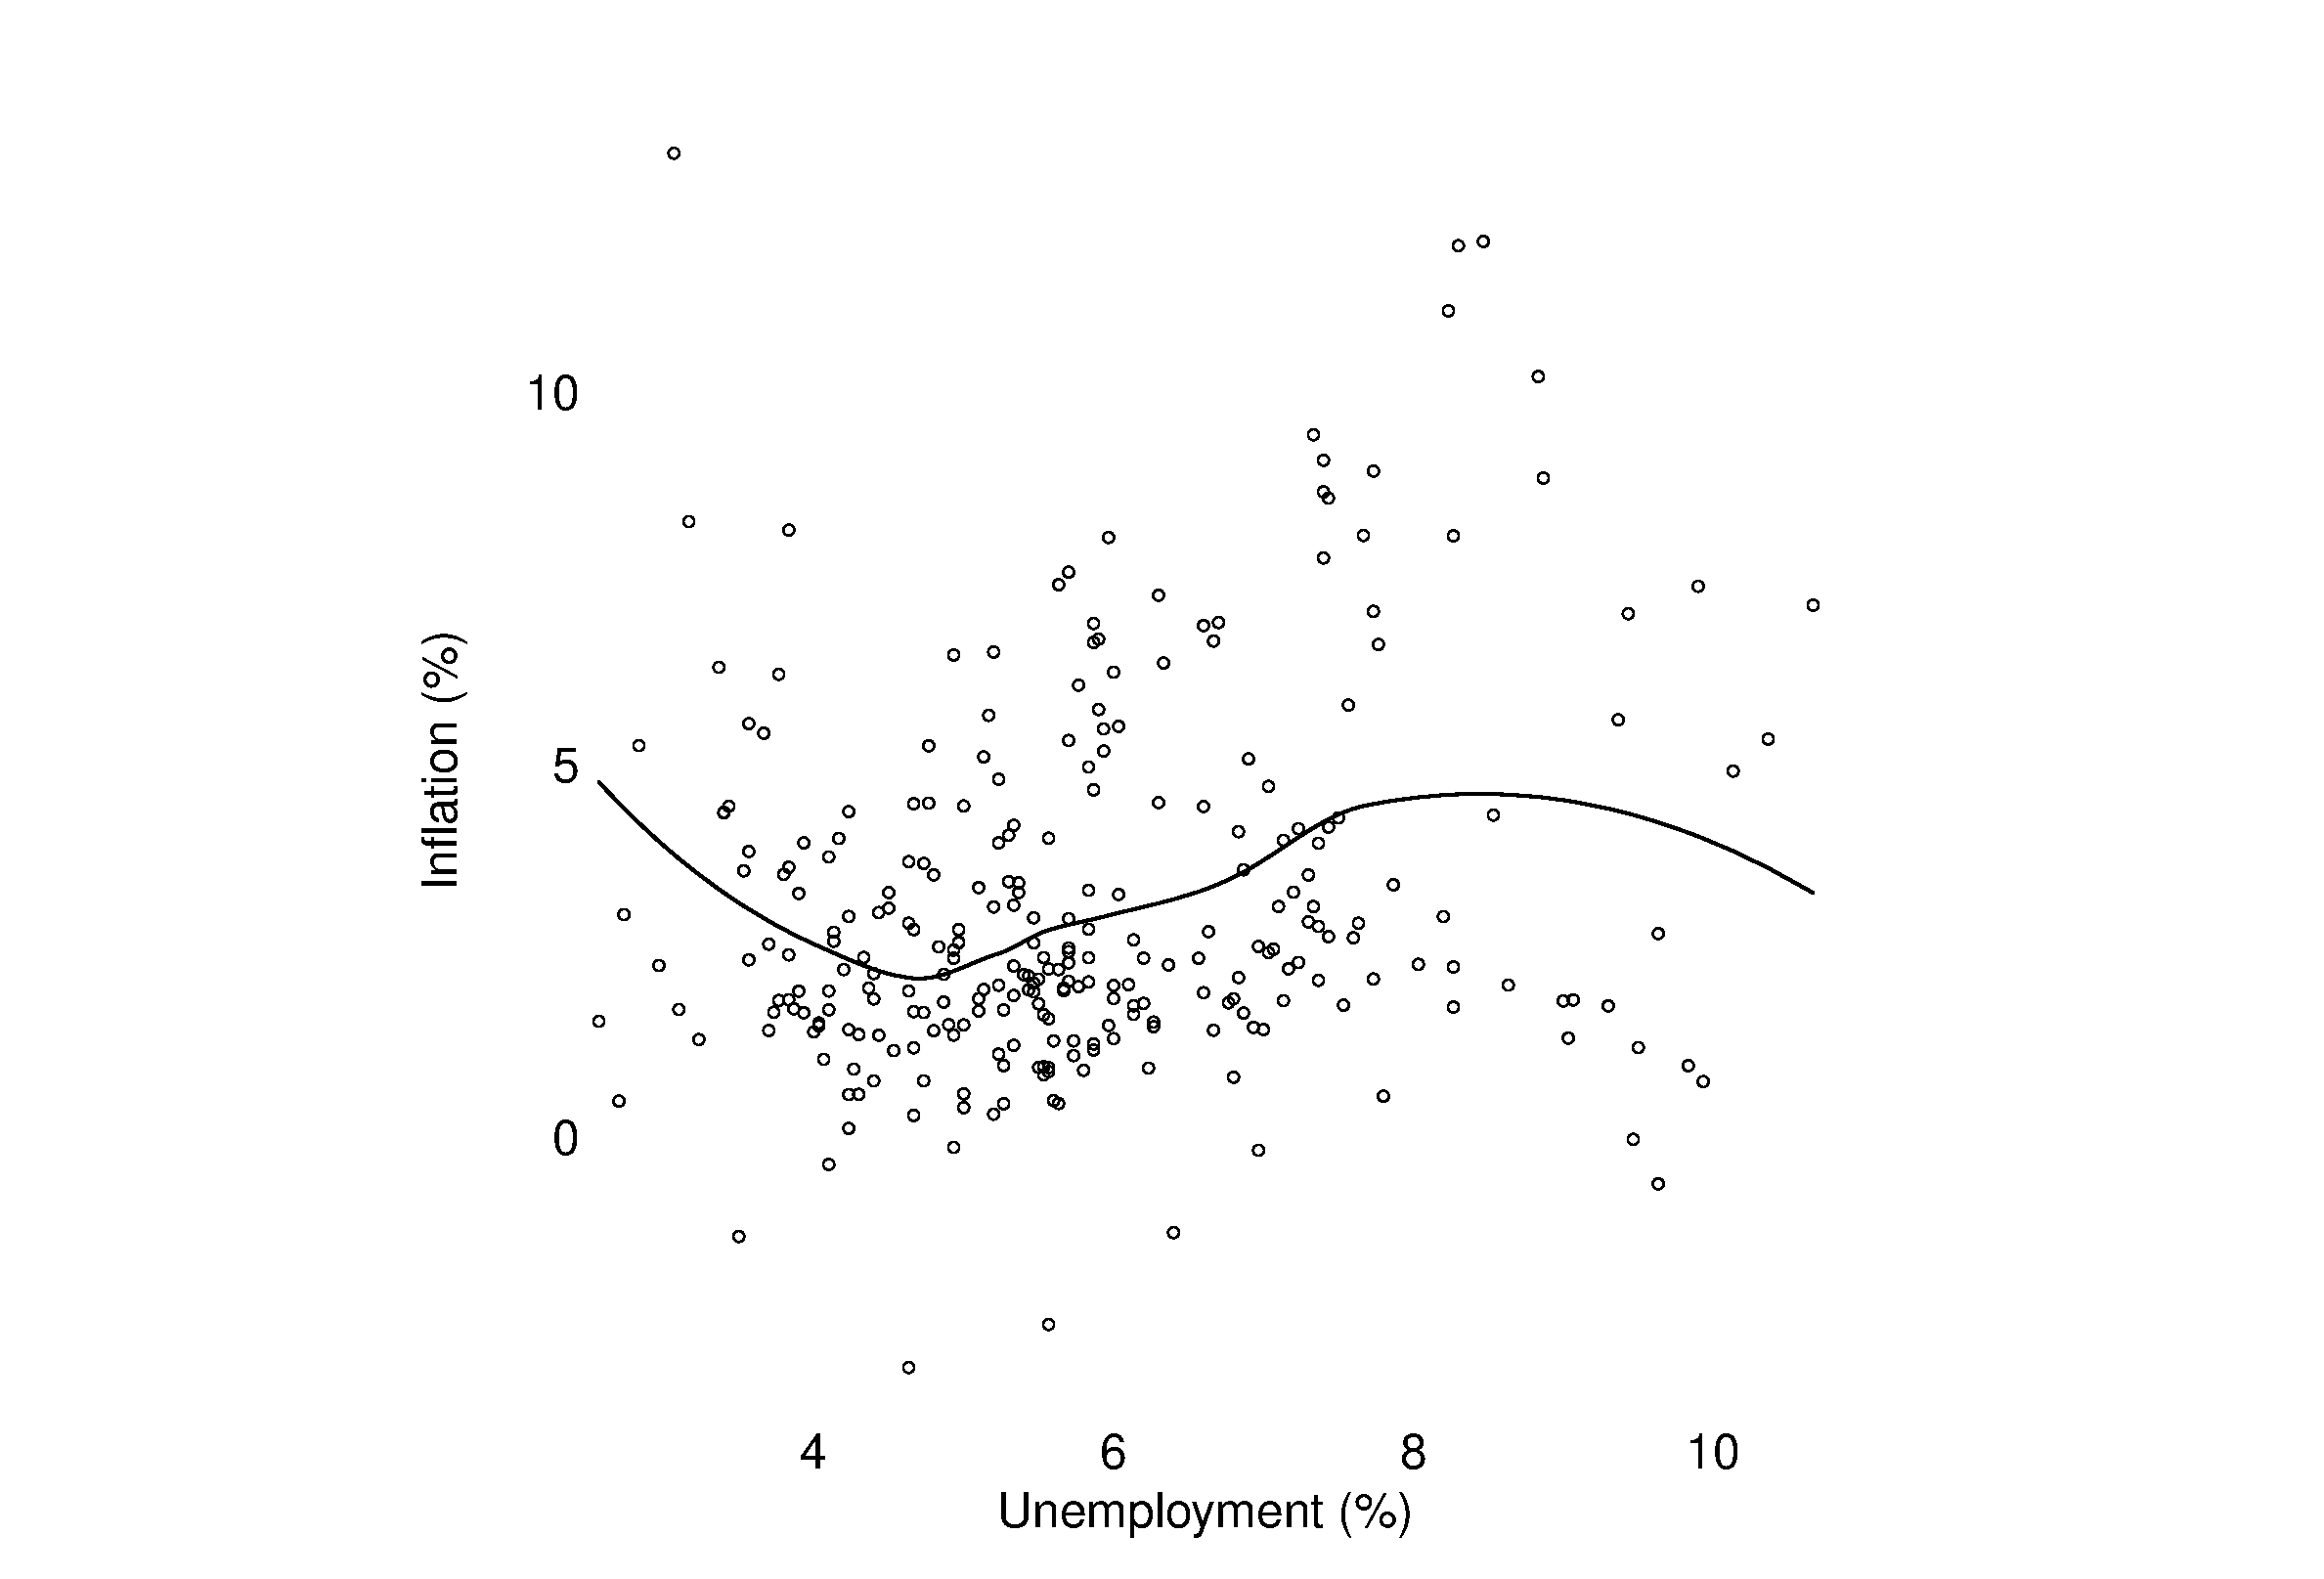
\includegraphics[scale=.25]{pc6.eps}
  \end{figure}
\end{frame}
%--------------------------------------

%--------------------------------------
\begin{frame}
  Peterson Institute conference
  \begin{itemize}
    \item Blanchard: still exists, hard to pin down
    \item Summers: agnostic
    \item Draghi: ...
  \end{itemize}
\end{frame}
%--------------------------------------

%--------------------------------------
\begin{frame}
\textbf{Friedman:}
 \begin{align}
   \pi_t = \mathbb{E}\pi_t -\gamma(U_t-U^*) 
 \end{align}
 In long run
 \begin{align}
   \mathbb{E}\pi_t \approx \pi_t
 \end{align}
 i.e. $U_t \approx U^*$
\end{frame}
%--------------------------------------

%--------------------------------------
\begin{frame}
  \textbf{Accelerationist Phillips curve}
  \begin{align}
    \mathbb{E}\pi_t=\pi_{t-1}\\
    \pi_t=\pi_{t-1} -\gamma(U_t-U^*)
  \end{align}
  \begin{enumerate}
    \item $U _t < U^*$: increase in $\pi$
    \item $U _t > U^*$: decrease in $\pi$
  \end{enumerate}
  
  
\end{frame}
%--------------------------------------

%--------------------------------------
\begin{frame}
\textbf{Non-accelerating Inflation Rate of Unemployment} (NAIRU)
  \begin{align}
    \pi_t= \sum_{i=1}^N \beta_i\pi_{t-i} -\gamma(U_t-U^*)
  \end{align}  
  $U^*$ is unknown but can be estimated
\begin{align}
  \pi_t &=\alpha - \gamma U_t +\sum_{i=1}^N \beta_i \pi_{t-i}\\
  \alpha - \gamma U^* &= 0 \Rightarrow  U^* = \frac{\alpha}{\gamma}  
\end{align}
\end{frame}
%--------------------------------------

%--------------------------------------
\begin{frame}
Implications for policy analysis
\begin{enumerate}
  \item Inflation: highly inertial; shock $t$ takes long time to disappear
  \item \begin{align} \mathbb{E}\pi_t=\pi_{t-1}  \end{align}
  Backward-looking: hard to decrease $\pi$ without increase $U$
\end{enumerate}
\medskip
Best course of action: let monetary policy reduce $\pi$ gradually over time
\end{frame}
%--------------------------------------


%--------------------------------------
\begin{frame}
  \textbf{Critique of Keynesianism}
  \begin{align}
  \pi_t = \mathbb{E}\pi_t - \gamma (U_t - U^*) 
\end{align}
Can have $U_t \neq U^*$ only when there is unexpected inflation
\begin{itemize}
  \item $\pi_t \neq E\pi_t$
\end{itemize}
  IF expectations are rational, then
  \begin{itemize}
    \item Unexpected inflation is random and unpredictable
    \item No room for systematic predictable stabilisation 
    \begin{itemize}
      \item No PC; little central bank can do
    \end{itemize}
  \end{itemize}
RE advocates believed that monetary policy had little to do with business cycles
\end{frame}
%--------------------------------------

%--------------------------------------
\begin{frame}
  Blanchard et al. (2015)
  \begin{align}
    \pi_t &= \theta_t(u_t-u^*_t) + \lambda_t\pi_t^e + (1-\lambda_t)\pi_{t-1}^* + \mu_t\pi_{mt} + \epsilon_t\\
    \pi_t^e &= a_t + \beta_t\pi_{t-1}^* + \eta_t
  \end{align}
  \medskip
  Inflation determined by unemployment, but also by
  \begin{enumerate}
    \item Inflation expectations
    \item Inflation history
    \item Import prices
    \item Random shock
  \end{enumerate}
\end{frame}
%--------------------------------------


%--------------------------------------
\begin{frame}
  \begin{figure}
   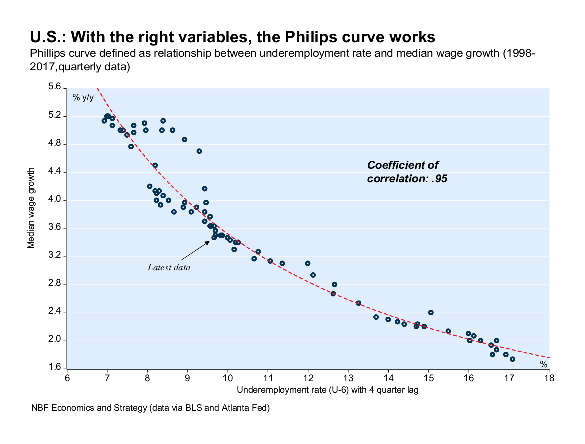
\includegraphics[scale=.8]{pc5.eps}
  \end{figure}
\end{frame}
%--------------------------------------

%--------------------------------------
\begin{frame}
  \begin{figure}
   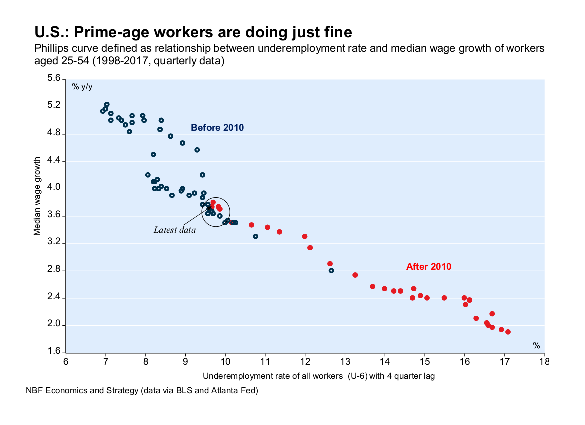
\includegraphics[scale=.8]{pc4.eps}
  \end{figure}
\end{frame}
%--------------------------------------


%--------------------------------------
\end{document}
